In this section the design of the trajectory followed by the spacecraft during the mission is presented. Also the motivation behind it, its sensitivity to changing atmospheric properties and the possibility to correct for these changes are explained. The main input with which the trajectory is calculated is the shape of the decelerator. This shape and the reasoning behind it is presented in Section \ref{sec:AeroDesign}. An overview of the mission trajectory is given in Figure \ref{fig:trajectory}.

\paragraph{Aerocapture}
The first phase of the trajectory is aerocapture, in this phase the objective is to loose enough energy to get in a Mars synchronous orbit. The velocity that has to be obtained at the end of aerocapture in order to get in such an orbit is $4.53 \left[km \cdot s^{-1}\right]$. In Figure \ref{fig:orbit_aerocapture_data} it can be seen from the velocity profiles that they all end at this velocity.

Furthermore the trajectory was chosen as high through the atmosphere as possible to facilitate \gls{tps} and structural masses. A pass higher through the atmosphere decreases both the heat flux and peak dynamic pressure which are used to design the \gls{tps} and inflatable structure respectively.

These two objectives are conflicting as the deceleration high in the atmosphere is often too low to achieve the required velocity change. In order to still reach the desired velocity, the duration of the aerocapture, the drag coefficient or the area of the decelerator has to be increased. 

A longer aerocapture can be achieved by improved control over the vehicle, which is accomplished by a higher lift coefficient.  A longer aerocapture, however increases the heat flux. 

With a higher drag coefficient or area the vehicle can obtain a larger deceleration higher in the atmosphere, thus at a lower dynamic pressure. In order to facilitate both our objectives it is thus important that the aerodynamic shape created has a high lift coefficient as well as a high drag coefficient.

In figure \ref{fig:orbit_aerocapture_data} the parameters that were recorded during the simulation are shown for the nominal trajectory and two trajectories created for a 10 \% increase and decrease in atmospheric density. This change in density is based on the maximum estimated error in the ESA mars climate database v5.2 \cite{Lewis2015}.

The bank control for the trajectories is changed to attain the same exit velocity. This velocity is needed to get into a Mars synchronous orbit. With this results it is proven that a density change of $\pm 10\%$ can be accounted for by changing the bank control. However, some other parameters do change. The peak acceleration and dynamic pressure increase for a higher density. The \gls{tps} and inflatable structure should be sized on the worst case. Also the time passed and the position of exit (defined by $\theta$) are different for the different trajectories. These changes have a significant effect on the entry and descent phase.
\begin{sidewaysfigure}
	\centering
	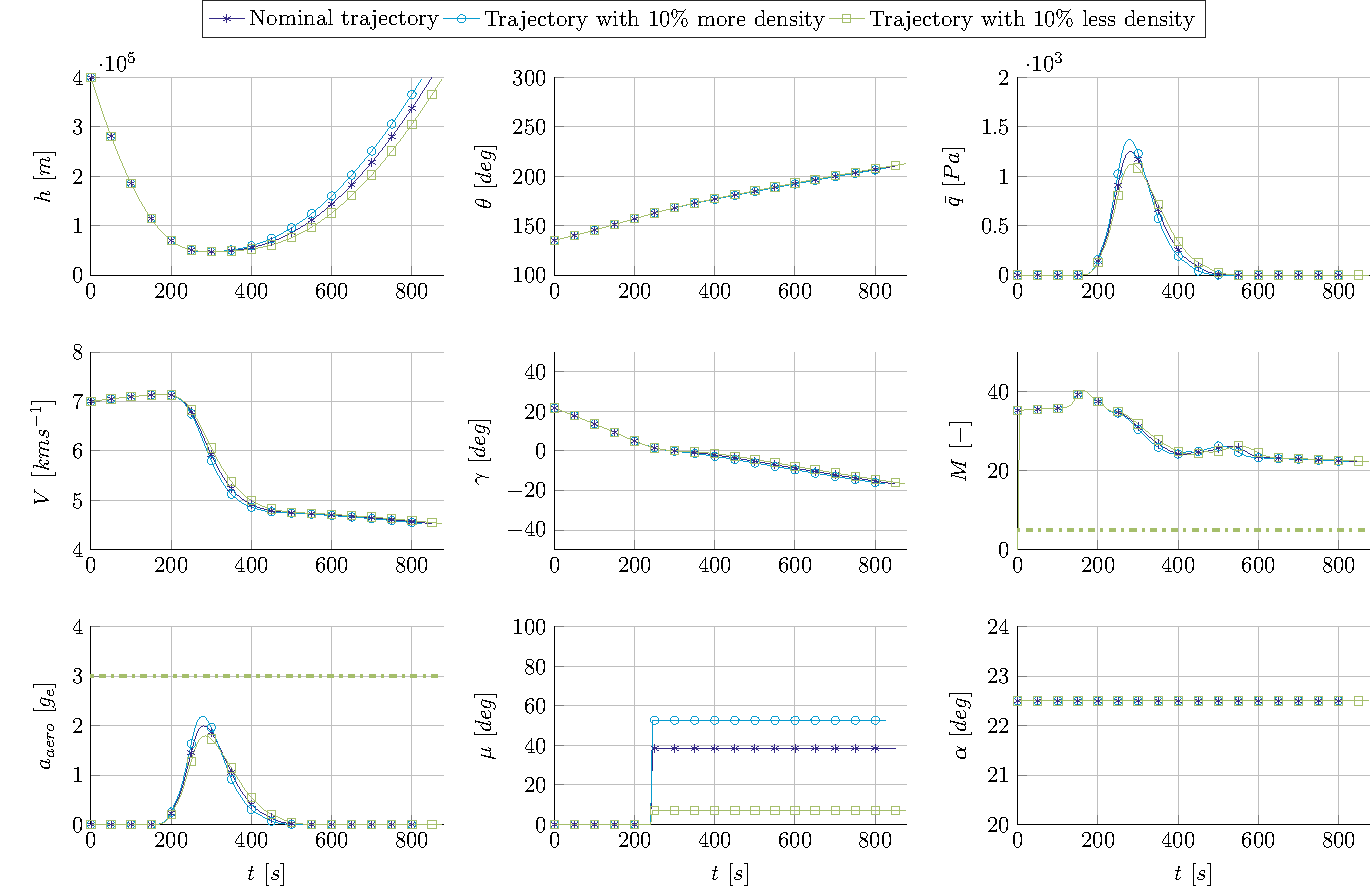
\includegraphics[width=0.99\textwidth]{Figure/Orbit/sensitivity_aerocapture.pdf}
	\caption{Results of the aerocapture trajectory for three different density profiles. The trajectories with modified density are corrected (changed \gls{sym:mu} profile) to maintain the same exit velocity. The horizontal dashed lines are design limits (for the \gls{sym:M} and \gls{sym:acc} plots) }
	\label{fig:orbit_aerocapture_data}
\end{sidewaysfigure}

\paragraph{Parking orbit}
After aerocapture the spacecraft goes into an eliptic orbit. In the apoareion (apocenter of an orbit around mars) a boost is given to raise the periareion to $200 \left[km\right]$ above \gls{mola}. In this parking orbit the vehicle can wait for dust storms to vanish and can observe the entry conditions it wil be subjected to. Because the parking orbit is mars synchronous the point observed is the same and changes can be accurately observed at the entry location. 

The first entry opportunity is after approximately two earth days from the start of the mission. From that moment every sol an opportunity for entry arises. This gives in total eight opportunites for entry in little over nine earth days. This is the maximum that can be achieved within the ten days that are available for the mission. In principle the spacecraft could stay in the parking orbit much longer if it would be necessary. However the current mission is fully designed for an entry of at most 10 days. i.e. crew operational items are insufficient to sustain a longer mission.

For every entry opportunity the decision to start entry has to be made approximately half a sol before the entry. In the apoareion a boost opposite to the flight direction should be given to lower periareion of the orbit.  When the vehicle reaches the atmosphere in this lower orbit the entry and descent pahse begins. 

\paragraph{Entry and descent}
The boost given in the apoareion before entry is determined such that the initial flight path angle of the entry is $-17.2 \left[deg\right]$. 

***Entry conditions imposed by aerocapture and parking orbit***\\
***trajectory based on 3g requirement \& Mach 5 requirement***\\
***$\alpha$ control not necessary***\\

***Sensitivity to density change +-10\% and possibility to correct for it***\\
\begin{sidewaysfigure}
	\centering
	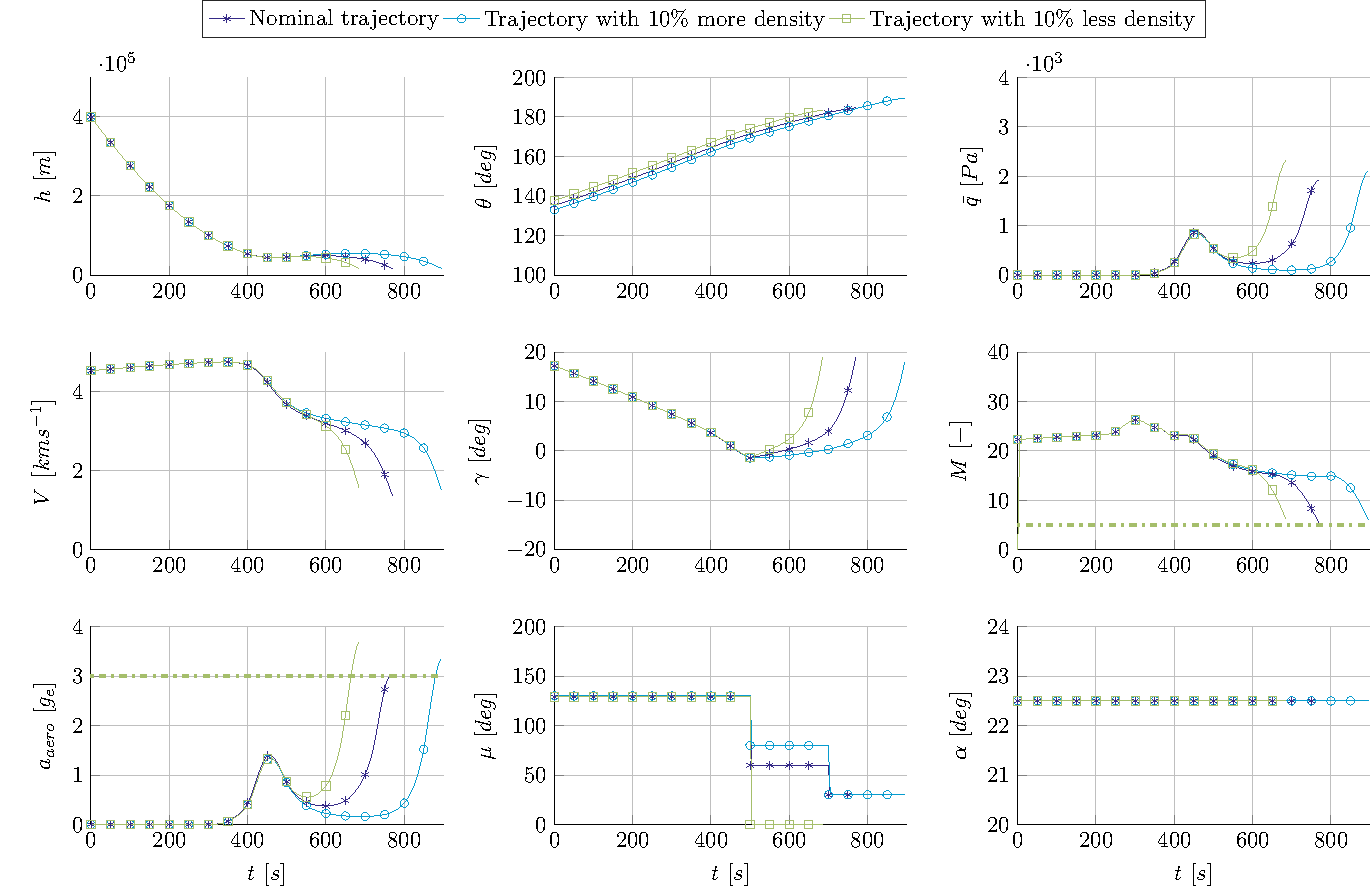
\includegraphics[width=0.99\textwidth]{Figure/Orbit/sensitivity_entry.pdf}
	\caption{Results of the re-entry trajectory for three different density profiles. The trajectories with modified density are corrected (changed \gls{sym:mu} profile) to show the ability to reach the desired landing location. The horizontal dashed lines are design limits (for the \gls{sym:M} and \gls{sym:acc} plots)}
	\label{fig:orbit_entry_data}
\end{sidewaysfigure}

\begin{figure}[h]
	\centering
	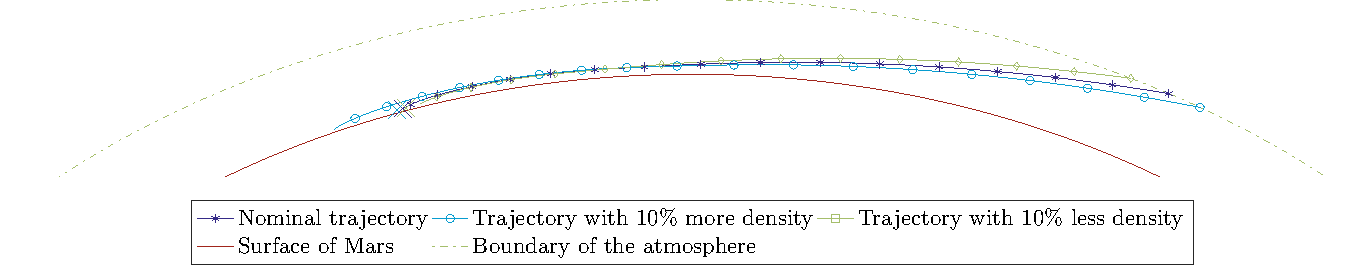
\includegraphics[width=0.99\textwidth]{Figure/Orbit/entry_mars.pdf}
	\caption{The re-entry trajectory for three different density profiles. The trajectories with modified density are corrected (changed \gls{sym:mu} profile) to show the ability to reach the desired landing location.}
	\label{fig:entry_mars}
\end{figure}

\begin{figure}
	\centering

	\begin{subfigure}[b]{0.7\textwidth}
		\vspace{-22mm}
		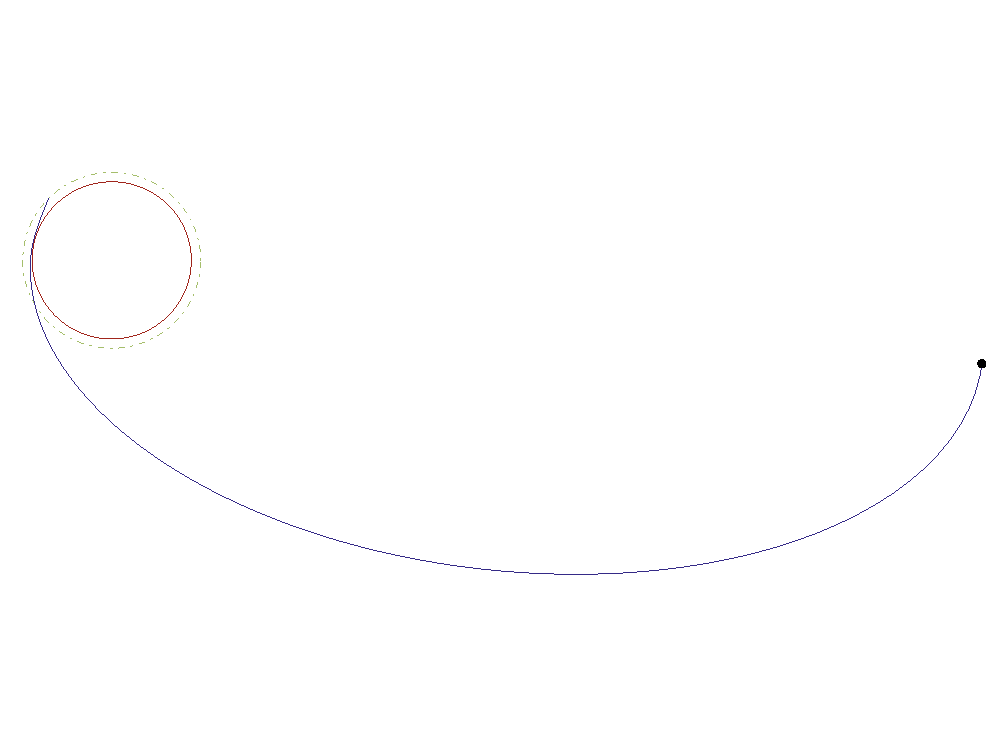
\includegraphics[width=\textwidth]{./Figure/Orbit/aerocapture_trajectory.pdf}
		\vspace{-25mm}
		\caption{The aerocapture trajectory visualized.}
		\label{fig:capture_trajectory}
	\end{subfigure}
	\begin{subfigure}[b]{0.7\textwidth}
		\vspace{-10mm}
		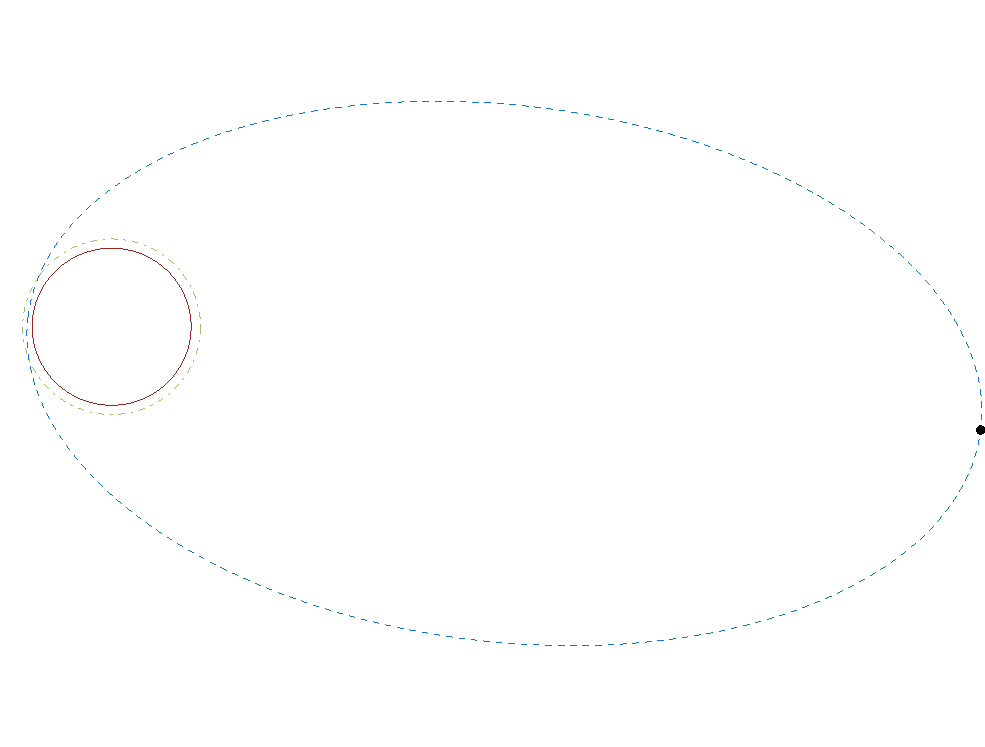
\includegraphics[width=\textwidth]{./Figure/Orbit/parking_trajectory.pdf}
		\vspace{-15mm}
		\caption{The parking orbit after the orbit raise}
		\label{fig:parking_trajectory}
	\end{subfigure}
	\begin{subfigure}[b]{0.7\textwidth}
		\vspace{-22mm}
		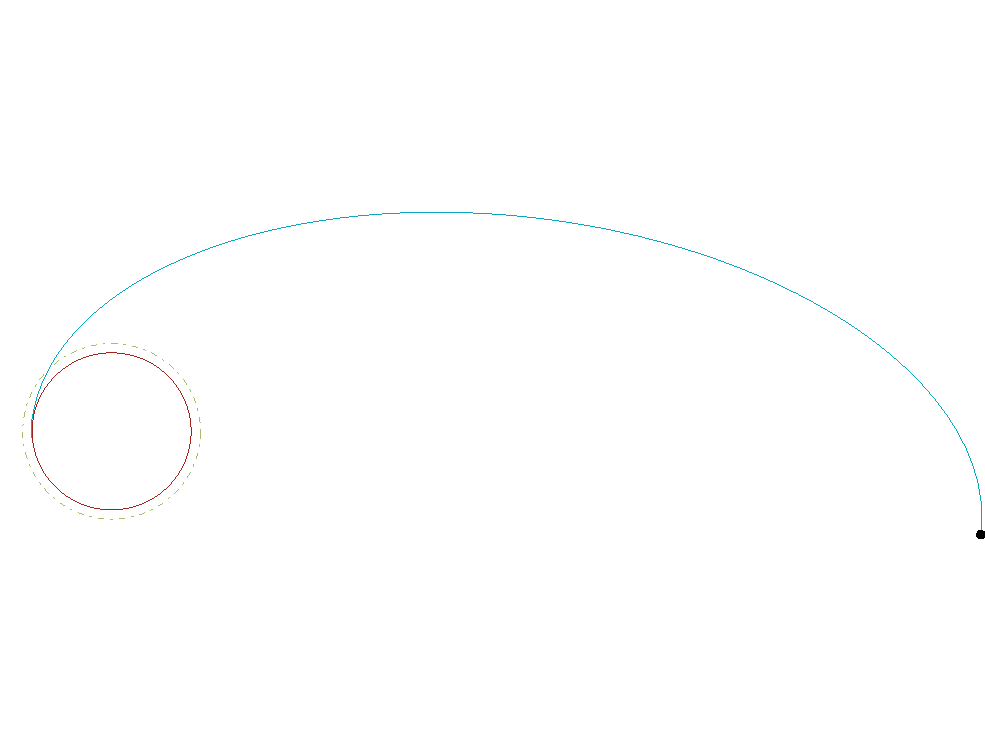
\includegraphics[width=\textwidth]{./Figure/Orbit/re-entry_trajectory.pdf}
		\vspace{-25mm}
		\caption{The re-entry trajectory after lowering the orbit.}
		\label{fig:re_entry_trajectory}
	\end{subfigure}
	\caption{The trajcetory of the spacecraft visualized. The apoareion is shown with a black dot.}
	\label{fig:trajectory}
\end{figure}
